% !TeX spellcheck = cs_CZ
\begin{mdframed}[style=mdexam]
  \begin{example}\label{cpp:exam002}
    Tento program předvádí \lstinline[basicstyle=\ttfamily]!myclass!, popsanou výše v textu. 
    Nastavuje hodnoty \lstinline[basicstyle=\ttfamily]!a! pro 
    \lstinline[basicstyle=\ttfamily]!ob1! a 
    \lstinline[basicstyle=\ttfamily]!ob2!, a pak zobrazuje hodnotu a pro každý objekt.
    % \marginpar{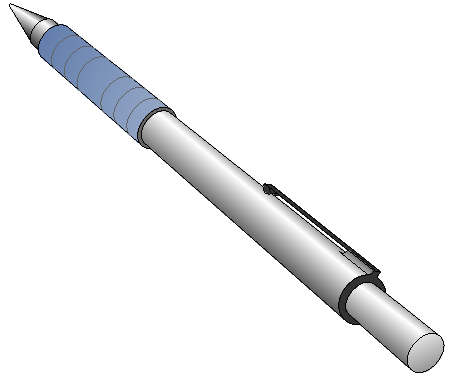
\includegraphics[width=0.05\textwidth]{pen.pdf}}
    \vspace{1em}       
    %---------------------------------------------------------------
    \lstinputlisting[style=luaCPPStyle, caption={\texttt{HS\_37\_myclass.cpp}: představení třídy 
    \texttt{myclass}.}]{../src/CES/CPP/HS_37_myclass.cpp}
    %---------------------------------------------------------------
    Program by měl na obrazovce zobrazit hodnoty \lstinline[basicstyle=\ttfamily]!10! a 
    \lstinline[basicstyle=\ttfamily]!99!.
  \end{example}
\end{mdframed}